\documentclass[10pt]{ctexbeamer}
\usepackage{bm}
\usepackage{tikz}
\usepackage{amsmath}
\usepackage{graphicx}
\newfontfamily{\dengxian}{DengXian}
\newCJKfontfamily{\fzyaoti}{FZYaoTi} %方正姚体
\newCJKfontfamily{\fzjinghong}{FZZJ-JHTJW} %方正字迹-惊鸿体
\newCJKfontfamily{\dqheiti}{Hiragino Sans GB} %冬青黑体
\newCJKfontfamily{\fandolhei}{FandolHei}

% \usetheme[color blocks]{Verona}% 使用Verona主题
% \usetheme[color blocks, red]{Verona}% 使用Verona主题, red theme
% \usetheme[color blocks, gray]{Verona}% 使用Verona主题, grey theme
\usefonttheme[onlymath]{serif}% 数学公式字体设置
\author{Norsesun}
\date{最后更新:\today}
\logo{
\includegraphics[height=1.2cm]{../../../Pngtree owl double exposure.png}}

\definecolor{airforceblue}{rgb}{.36,.54,.66}



\newcommand{\bmc}[1]{$\bm{#1}$}%定义一个新命令,行内数学模式的粗体,使幻灯片上的公式更清楚
\newcommand{\bmcc}[1]{
        \begin{displaymath}
            \bm{#1}
        \end{displaymath}
    }%定义一个新命令,行间数学模式的粗体,使幻灯片上的公式更清楚
\newcommand{\makecenter}[1]{\vspace{0.5em}\centering \parbox{.6\textwidth}{#1}}%定义一个新命令,居中排布一段话
\newenvironment{Mathbreakcenter}[1][1mm]{
        \par
        \vspace{#1} 
        \centering

    }{
        \par
        \vspace{2mm}
    }
\newcommand{\myblock}[3][1-]{
    \centering
    \begin{minipage}{.6\textwidth}
        \begin{block}<#1>{#2}%
            \centering%
            #3
        \end{block}
    \end{minipage}  
    } %定义一个新命令,居中排布一个block

    \newcommand{\myalertblock}[3][1-]{
        \centering
        \begin{minipage}{.6\textwidth}
            \begin{alertblock}<#1>{#2}%
                \centering%
                #3
            \end{alertblock}
        \end{minipage}  
        } %定义一个新命令,居中排布一个alertblock
\newcommand{\cleave}[2]{
    \hbox to #1{} #2 \hbox to #1{}
}
% \newcommand{\annmark}[1]{%
%     \textcolor{red}{$\bm\langle$#1$\bm\rangle$}%
% }%

% \newcommand{\ann}[1]{%
%     \begin{tikzpicture}[remember picture, baseline=-0.75ex]%
%         \node[coordinate] (inText) {};%
%     \end{tikzpicture}%
%     \marginpar{%
%         \renewcommand{\baselinestretch}{1.0}%
%         \begin{tikzpicture}[remember picture]%
%             \definecolor{orange}{rgb}{1,0.5,0}%
%             \draw node[fill=red!20,rounded corners,text width=\marginparwidth] (inNote){\footnotesize#1};%
%     \end{tikzpicture}%
%     }%
%     \begin{tikzpicture}[remember picture, overlay]%
%         \draw[draw = orange, thick]
%             ([yshift=-0.2cm] inText)
%                 -| ([xshift=-0.2cm] inNote.west)
%                 -| (inNote.west);%
%     \end{tikzpicture}%
% }%

% \setlength{\marginparwidth}{2.5cm}
% \renewcommand{\baselinestretch}{1.3}

\newenvironment{mathsalvation}[2][{解:}]{
    \begin{center}{}
        \begin{minipage}[t]{.05\textwidth}
            \vspace{0pt}
            {\color{#2}{#1}} \quad 
        \end{minipage}
        \begin{minipage}[t]{.7\textwidth}
            \vspace{0pt}
            % \fzyaoti
            % \dengxian
            % \fzjinghong
            % \dqheiti
            \fandolhei
}{
    \end{minipage}
    \end{center}
}

\usepackage{wallpaper}
\usepackage{enumerate}

\title{等式的性质}
\subtitle{The nature of The Equality}
\AtBeginSubsection[]
{
	\begin{frame}{要点目录}
		\tableofcontents[currentsubsection]
	\end{frame}
}

\begin{document}
\frame{\titlepage}
\begin{frame}
    \begin{figure}[c]
        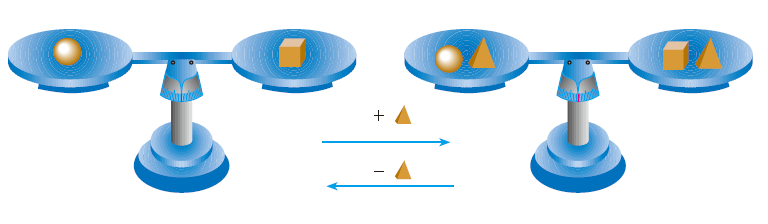
\includegraphics[width=.6\textwidth]{assets/tianping.png}
    \end{figure}
    \only<2>{
        \makecenter{从图中可以发现,如果在平衡的天平的两边都加(或减)同样的量,天平还保持平衡。}
    }
\end{frame}

\section{等式}
\subsection{等式性质1}
\begin{frame}
    \frametitle{天平与等式(Scale \& Equality)}
    \makecenter{把一个等式看作一个天平,把等号两边的式子看作天平两边的砝码,则等式成立就可看作是天平保持两边平衡。}
    \begin{figure}
        \includegraphics<1,2>[width=.6\textwidth]{assets/tianping2.png}
        \includegraphics<3->[width=.45\textwidth]{assets/scale.png}
    \end{figure}
    
    \myblock{2}{}{
        \bmc{
            a=b
        }
    }
    \myblock{3}{}{
        \bmc{
            a + c=b + c
        }
    }
\end{frame}

\begin{frame}
    \frametitle{等式性质1}
    \myblock{1-}{由等式 $ 1+2=3 $ 进行判断}{
        \centering
        \bmc{1 + 2 +4}
            \cleave{10mm}{\only<1>{?} \only<2>{=}}
        \bmc{3 +4} \\
        \bmc{1 + 2 -5}
            \cleave{10mm}{\only<1>{?} \only<2>{=}}
        \bmc{3 - 5}
    }

    \vspace{1cm}  
    \pause
    \makecenter{等式的两边同时\alert{加上(或减去)同一个数}所得的结果仍是等式. 
    }
\end{frame}

\begin{frame}
    \frametitle{等式性质1}
    \myblock{1-}{由等式 $ 2x+3x=5x $ 进行判断}{
        \centering
        \bmc{2x +3x + 4x}
            \cleave{10mm}{\only<1>{?} \only<2>{=}}
        \bmc{5x+4x} \\
        \bmc{2x +3x-x}
            \cleave{10mm}{\only<1>{?} \only<2>{=}}
        \bmc{5x -x }
    }

    \vspace{1cm}  
    \pause
    \makecenter{等式的两边同时\alert{加上(或减去)同一个式子}所得的结果仍是等式. 
    }
\end{frame}

\setbeamercolor{background canvas}{bg=teal}
\begin{frame}[plain]
    \myalertblock{1-}{等式性质1}{
        等式的两边同时加上(或减去)\alert{同一个数或同一个式子},
        所得的结果仍是等式。
        \vspace{1em}

        \only<2>{若\bmc{a=b},则 \bmc{a + c = b + c}。}
    }
\end{frame}
\setbeamercolor{background canvas}{bg=white}

\subsection{等式性质1-练习}
\begin{frame}
    \frametitle{练习1}
    \makecenter{在下面的括号内填上适当的数或者式子:}
    \makecenter{
        \myblock{1}{}{
            \begin{itemize}
                \item 若 \bmc{2x-6=4}, \\
                则 \bmc{2x-6+6=4+(}
                    \hbox to 10mm{}
                    \bmc{)}
                \item 若 \bmc{3x=2x-8}, \\
                则 \bmc{3x+(}
                    \hbox to 10mm{}
                    \bmc{)=2x-8-2x}
                \item 若 \bmc{10x-9=8-6x}, \\
                则\\ \bmc{10x+(}
                    \hbox to 2mm{}
                    \bmc{)-9+9=8-6x+6x+(}
                    \hbox to 2mm{}
                    \bmc{)}
            \end{itemize}
        } 
    }
\end{frame}

\subsection{等式性质2}
\begin{frame}{等式性质2}
    \begin{figure}
        \includegraphics<1, 2>[width=.6\textwidth]{assets/scale2.png}
        \includegraphics<3->[width=.6\textwidth]{assets/scale3.png}

        已知\bmc{a=b}
    \end{figure}

    \myblock{2-}{}{
        \only<2>{\bmc{a + a + a = b + b + b}

        \bmc{3a = 3b}}

        \only<3->{\bmc{ac = bc}}

        
        \only<4>{\vspace{1em}\bmc{ \dfrac{a}{c} = \dfrac{b}{c}} (\bmc{c \neq 0})}
    }
\end{frame}

\begin{frame}
    \frametitle{等式性质2}
    \myblock{1-}{由等式 $ 3m+5m=8m $ 进行判断}{
        \centering
        \bmc{2 \times (3m+5m)}
            \cleave{10mm}{\only<1>{?} \only<2>{=}}
        \bmc{2 \times 8m} \\
        \vspace{1cm} 
        \bmc{\dfrac{3m + 5m}{2}}
            \cleave{10mm}{\only<1>{?} \only<2>{=}}
        \bmc{\dfrac{3m}{2}}
    }
\end{frame}

\setbeamercolor{background canvas}{bg=teal}
\begin{frame}[plain]
    \myalertblock{1-}{等式性质2}{
        等式的两边同时\alert{乘同一个数},或\alert{除以同一个不为
        \bmc{0}的数}
        所得的结果仍相等。
        \vspace{1em}

        \only<2>{
            若\bmc{a=b},则 \bmc{ac = bc}
            
            若\bmc{a=b, c\neq 0},则 \bmc{ \dfrac{a}{c} = \dfrac{b}{c}}
        }
    }
\end{frame}
\setbeamercolor{background canvas}{bg=white}

\subsection{等式性质2-练习}
\begin{frame}
    \frametitle{练习2}
    \makecenter{怎样从等式 \bmc{4x=12} 得到等式 \bmc{x =3}?}
    \vspace{1em}
    \makecenter{
        怎样从等式 \bmc{\dfrac{a}{100}} 得到等式 \bmc{a = b}?
    }
\end{frame}

\begin{frame}
    \frametitle{练习3}
    \makecenter{已知\bmc{mx=my},下列结论错误的是(\hbox to 4mm{\only<2>{ A}})}
    \myblock{1-}{}{
        \begin{enumerate}[(A)]
            \item \bmc{x=y}
            \item \bmc{a+mx=a+my}
            \item \bmc{mx-y=my-y}
            \item \bmc{amx=amy}
        \end{enumerate}
    }
\end{frame}

\begin{frame}
    \frametitle{练习4}
    \makecenter{已知\bmc{x=y},判断下列结论的对错,并说明原因}
    \myblock{1-}{}{
        \begin{enumerate}[(I)]
            \item \bmc{x - \frac{2}{3} = y + \frac{2}{3}}
            \item \bmc{x+5-a=y+5-a}
            \item $\dfrac{\bm{x}}{\bm{5-a}} =\dfrac{\bm{y}}{\bm{5-a}} $
                \begin{flushright}
                    \only<2>{\color{red}{\normalsize 错, $a=5$时无意义}}
                \end{flushright}
            \item \bmc{-5x=5y}
            \item \bmc{2x-\frac{1}{3}=2y-\frac{1}{3}}
        \end{enumerate}
    }
\end{frame}

\section{利用等式性质解方程}
\begin{frame}
    \frametitle{利用等式性质解方程}
    \makecenter{利用等式的性质解下列方程}
    \myblock{1-}{}{
        \begin{enumerate}[i]
            \item \bmc{x+7=26}
            \item \bmc{-5x=20}
            \item \bmc{-\dfrac{1}{3}x-5=4}
        \end{enumerate} 
    }
    \only<2>{
        \begin{description}
            \item[解:] 第一个方程两边同时减去$7$, 得:
                \begin{align}
                    \bm{x +7 -7 = 26 -7} \\
                    \bm{x=19}
                \end{align}
        \end{description}
    }
    \only<2>{
        \myblock{2}{}{解一元一次方程要 化归 为 \alert{$x=a$(常数)}的形式.
        }
    }
\end{frame}

\begin{frame}{检验方程的解}
    \makecenter{
        一般地,从方程解出未知数的值以后,可以代入原方程检验,
        看这个值能否使方程的两边相等。
    }
    \myblock{1-}{例如}{
        将$x=-27$ 带入方程 \bmc{-\dfrac{1}{3}x-5=4}的左边,\\
        \bmc{-\dfrac{1}{3}\times (-27)-5 = 9-5 = 4}\\
        \vspace{1em}
        方程左右两边相等,所以 $x=27$是原方程的解。
    }
\end{frame}
    
\begin{frame}
    \begin{figure}
        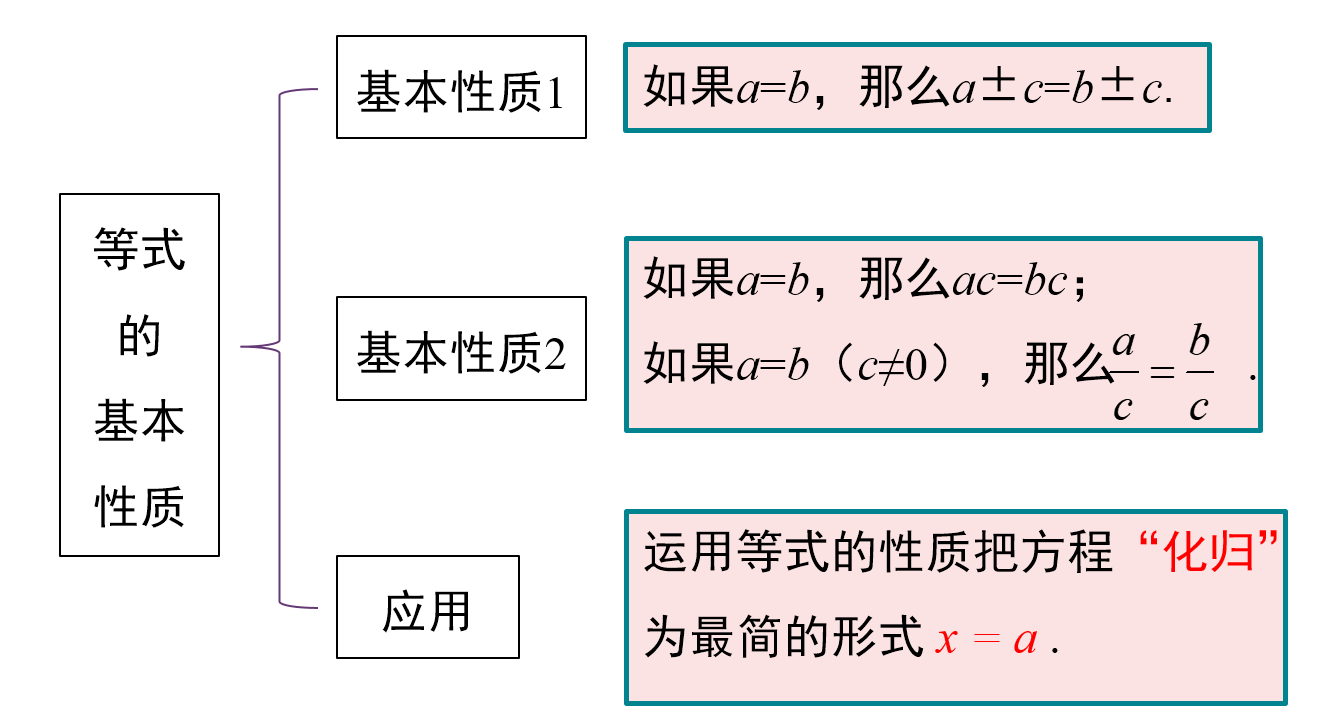
\includegraphics[width=.7\textwidth]{assets/conclusion1.png}
    \end{figure}
\end{frame}
\end{document}